% ---
% Capa
% ---
\imprimircapa
% ---

% ---
% Folha de rosto
% (o * indica que haverá a ficha bibliográfica)
% ---
\imprimirfolhaderosto*
% ---

% ---
% Inserir a ficha bibliografica
% ---
% http://ficha.bu.ufsc.br/
\begin{fichacatalografica}
	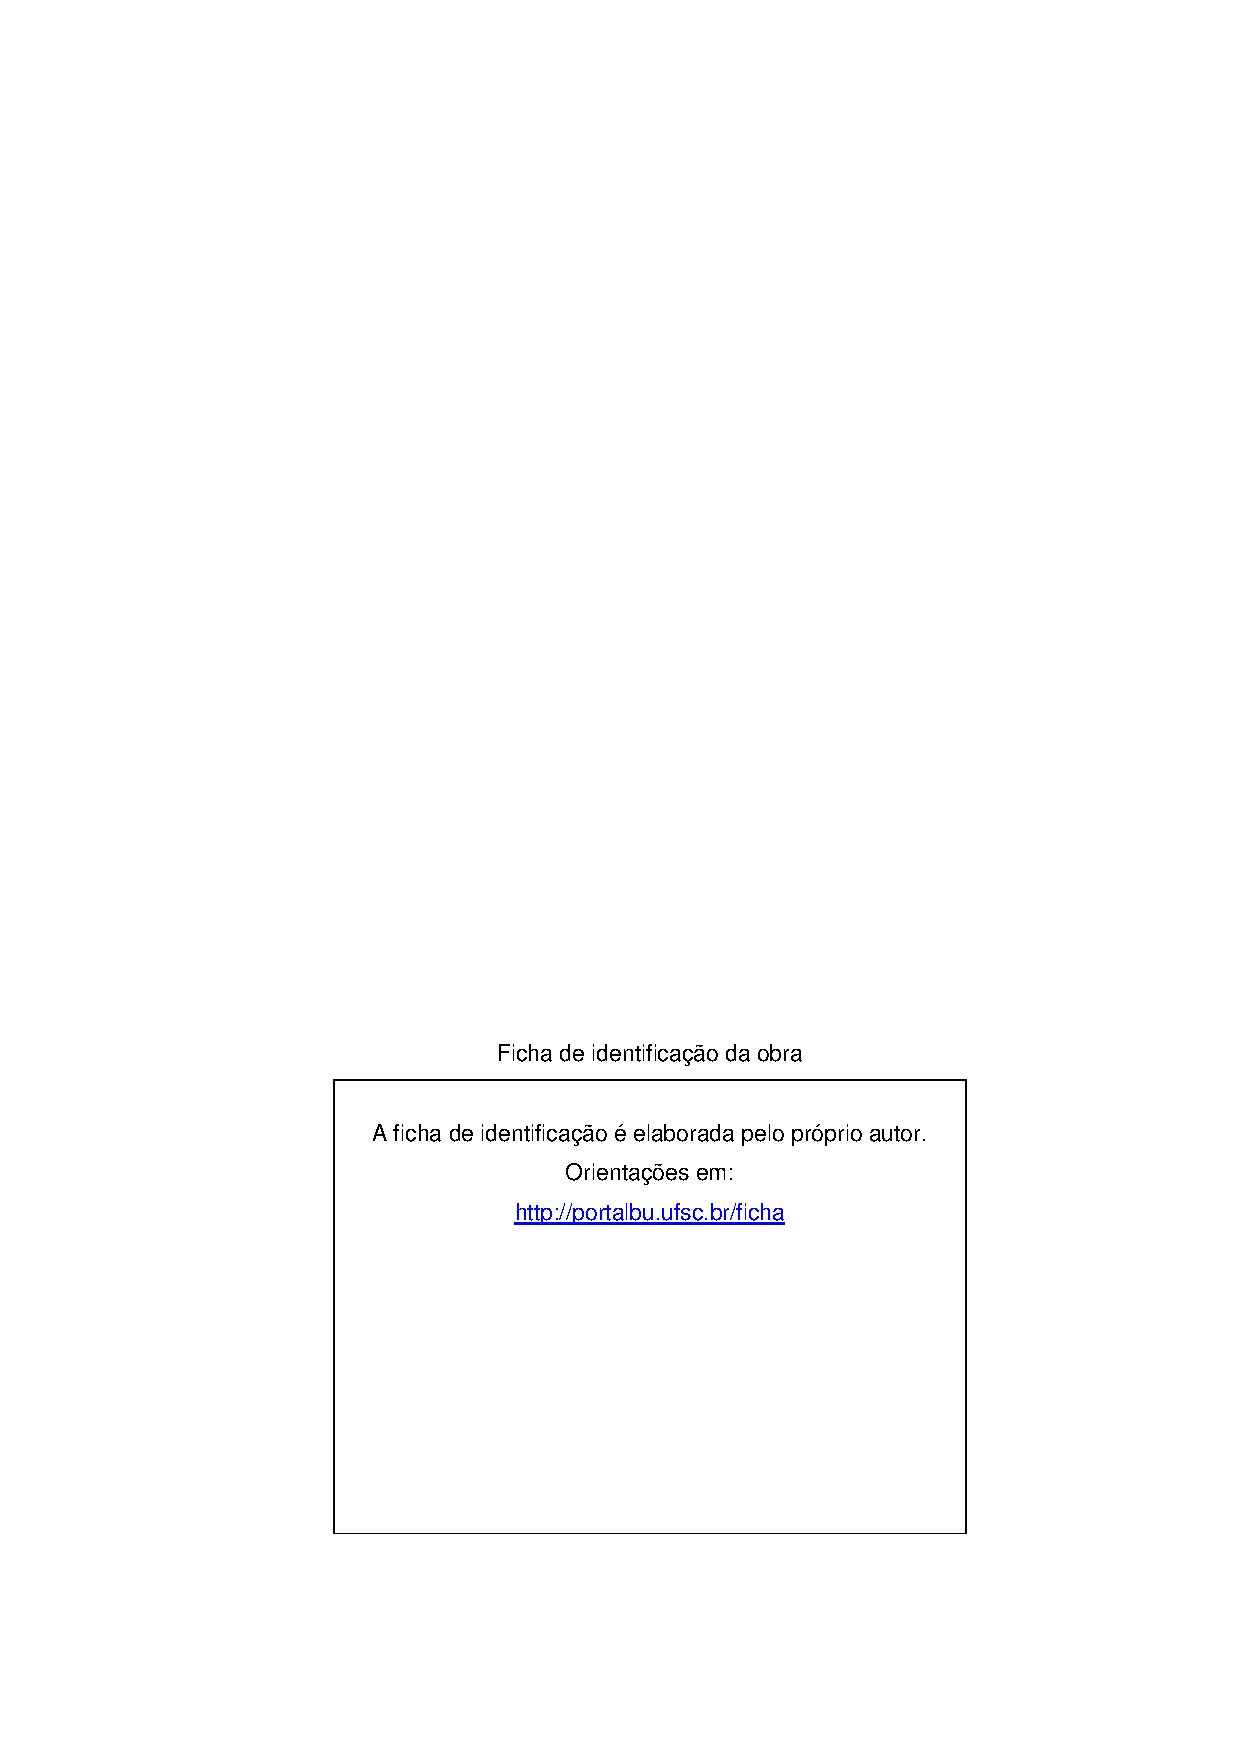
\includepdf{beforetext/Ficha_Catalografica.pdf}
\end{fichacatalografica}
% ---

% ---
% Inserir folha de aprovação
% ---
\begin{folhadeaprovacao}
	\OnehalfSpacing
	\centering
	\imprimirautor\\%
	\vspace*{10pt}		
	\textbf{\imprimirtitulo}%
	\ifnotempty{\imprimirsubtitulo}{:~\imprimirsubtitulo}\\%
	%		\vspace*{31.5pt}%3\baselineskip
	\vspace*{\baselineskip}
	%\begin{minipage}{\textwidth}
	% ~do~\imprimirprograma~do~\imprimircentro~da~\imprimirinstituicao~para~a~obtenção~do~título~de~\imprimirformacao.
	Este~\imprimirtipotrabalho~foi julgado adequado para obtenção do Título de “\imprimirformacao” e aprovado em sua forma final pelo~\imprimirprograma. \\
		\vspace*{\baselineskip}
	\imprimirlocal, \imprimirdata. \\
	\vspace*{2\baselineskip}
	\assinatura{\OnehalfSpacing\imprimircoordenador \\ \imprimircoordenadorRotulo~do Curso}
	\vspace*{2\baselineskip}
	\textbf{Banca Examinadora:} \\
	\vspace*{\baselineskip}
	\assinatura{\OnehalfSpacing\imprimirorientador \\ \imprimirorientadorRotulo}
	%\end{minipage}%
	\vspace*{\baselineskip}
	\assinatura{Prof. Pedro Luiz Borges Chaffe, Dr.\\
	Avaliador \\
	Universidade Federal de Santa Catarina}

	\vspace*{\baselineskip}
	\assinatura{Profa. Taciana Toledo de Almeida Albuquerque, Dra.\\
	Avaliadora \\
	Universidade Federal de Minas Gerais}

	\vspace*{\baselineskip}
	\assinatura{Prof. Thiago Nogueira, Dr.\\
	Avaliador \\
	Universidade de São Paulo}

	\vspace*{\baselineskip}
	\assinatura{Prof. Rizzieri Pedruzzi, Dr.\\
	Avaliador \\
	Universidade do Estado do Rio de Janeiro}

	\vspace*{\baselineskip}
	\assinatura{Prof. Alejandro Durán Carrillo de Albornoz, Dr.\\
	Avaliador \\
	Universidade de Havana, Cuba}

\end{folhadeaprovacao}
% ---

% ---
% Dedicatória
% ---
\begin{dedicatoria}
	\vspace*{\fill}
	\noindent
	\begin{adjustwidth*}{}{5.5cm}     
		Este trabalho é dedicado aos meus colegas de classe e aos meus queridos pais.
	\end{adjustwidth*}
\end{dedicatoria}
% ---

% ---
% Agradecimentos
% ---
\begin{agradecimentos}
	Inserir os agradecimentos aos colaboradores à execução do trabalho. 
	
	Xxxxxxxxxxxxxxxxxxxxxxxxxxxxxxxxxxxxxxxxxxxxxxxxxxxxxxxxxxxxxxxxxxxxxx. 
\end{agradecimentos}
% ---

% ---
% Epígrafe
% ---
\begin{epigrafe}
	\vspace*{\fill}
	\begin{flushright}
		\textit{``Texto da Epígrafe.\\
			Citação relativa ao tema do trabalho.\\
			É opcional. A epígrafe pode também aparecer\\
			na abertura de cada seção ou capítulo.\\
			Deve ser elaborada de acordo com a NBR 10520.''\\
			(Autor da epígrafe, ano)}
	\end{flushright}
\end{epigrafe}
% ---

% ---
% RESUMOS
% ---

% resumo em português
\setlength{\absparsep}{18pt} % ajusta o espaçamento dos parágrafos do resumo
\begin{resumo}
	\SingleSpacing
	O monitoramento da qualidade do ar tem experimentado uma mudança de paradigma com a incorporação de sensores de baixo custo. Estes equipamentos têm potencial para aumentar a resolução espaço-temporal dos dados de poluentes, assim como diversificar e simplificar as aplicações de monitoramento. Todavia, esses dispositivos ainda devem alcançar níveis de confiabilidade apropriados para serem utilizados de forma estendida. O volume e a diversidade de aplicações com este tipo de sensores encontra-se restrito pela baixa portabilidade de uma aplicação para outra e pela concentração de iniciativas maioritariamente em países desenvolvidos. No presente trabalho propõe-se uma solução para acelerar e facilitar o desenvolvimento e a diversificação de aplicações de monitoramento de baixo custo: a iniciativa CLEAN (Collaborative Low-cost Environmental Air quality Network). Ela consiste em uma rede colaborativa para o monitoramento de baixo custo da qualidade do ar. Os componentes da rede possuem uma arquitetura modularizada bem documentada, que possibilita o reaproveitamento de funcionalidades comuns entre aplicações. Dessa forma, os esforços de desenvolvimento podem ser direcionados à implementação dos requisitos específicos de cada aplicação particular. Dentro do marco da rede CLEAN foram desenvolvidos monitores de baixo custo. Um deles foi instalado junto a uma estação de monitoramento de referência da qualidade do ar, para validação e correção das suas leituras por um período de 5 meses. No trabalho propõe-se uma metodologia de correção das leituras do equipamento, a partir das medições coletadas pela estação de referência, utilizando modelos de regressão lineares e técnicas de aprendizado de máquinas. Durante a análise das medidas dos sensores, observou-se um alto índice de dados faltantes e alterações nos valores de linha base. Observou-se também uma correlação estatisticamente significativa entre os dados de temperatura e as leituras dos sensores de \acrshort{co}, \acrshort{o3} e \acrshort{mp10}, com coeficientes de Spearman entre 0.30 e 0.85. Os resultados obtidos nas correções, considerando as medidas de cada modelo de sensor isoladamente, foram positivos apenas nas medições de \acrshort{o3}, com um R2 máximo de aproximadamente 0.6 utilizando uma rede neural Perceptron Multicamadas e considerando a temperatura como variável de entrada no modelo. Para o restante dos sensores não foi encontrado nenhum modelo capaz de explicar a variância dos dados de concentração medidos pela estação de referência. Numa segunda iteração de processamento dos dados, aplicaram-se modelos de regressão que consideraram as leituras de todos os sensores para inferir as concentrações de um poluente. Para determinar os modelos foram testadas diferentes combinações de variáveis de entrada, técnicas de regressão e parâmetros dos modelos. As combinações que geraram os melhores resultados em termos de coeficientes de determinação foram selecionados para corrigir as leituras do equipamento de baixo custo. Dessa forma obteve-se uma melhoria nos resultados das regressões, com valores de R2 entre 0.03 e 0.5 entre todos os poluentes. A metodologia se mostrou suficientemente robusta para trabalhar com dados de baixa qualidade e acrescentar valor às leituras, sendo uma alternativa viável para equipamentos com leituras ruidosas ou falhas nos sensores. O trabalho traz como principais contribuições um marco de trabalho colaborativo para o desenvolvimento e interconexão de sensores de baixo custo, assim como uma metodologia para calibração dos sensores com dados muito ruidosos, em uma aplicação real e em ambiente não controlado.
	
	\textbf{Palavras-chave}: Monitoramento da qualidade do ar, rede colaborativa, sensores de gases de baixo custo, sistemas embarcados, \acrshort{api}, modelos de regressão, aprendizado de máquinas
\end{resumo}

% resumo em inglês
\begin{resumo}[Abstract]
	\SingleSpacing
	\begin{otherlanguage*}{english}
		Air quality monitoring has experienced a paradigm shift after incorporating  low-cost sensors. This equipments has a capability to increase the spatiotemporal resolution of pollutant data, as well as to diversify and simplify the monitoring applications. However, these devices must still reach appropriate reliability levels in order to extend its use. The volume and diversity of applications with this type of sensors is restricted by the low portability of one application to another and the concentration of initiatives mainly in developed countries. This work proposes a solution to accelerate and facilitate the development and diversification of low-cost monitoring applications: the CLEAN (Collaborative Low-cost Environmental Air Quality Network) initiative. It consists of a collaborative network for low-cost monitoring of air quality. The well documented modularized architecture of the network components allows the reusability of functionalities between applications. Thus, development efforts can be re-directed to implementing the specific requirements of each particular application. Within the framework of the CLEAN network, low-cost monitors were developed. A monitor was installed next to a certified station for monitoring air quality for a period of 5 months. This work proposes a methodology for correcting the readings of the equipment, based on measurements collected by the reference station and using linear regression models and machine learning techniques. During the analysis of sensor measurements, a high rate of missing data and changes in baseline values were observed. A statistically significant correlation was also observed between temperature data and sensor readings of \acrshort{co}, \acrshort{o3}, and \acrshort{mp10}, with Spearman coefficients between 0.30 and 0.85. The results obtained in the corrections, considering the measurements of each sensor model separately, were positive only for the measurements of \acrshort{o3}, with an R2 maximum of approximately 0.6 using a Multilayer Perceptron neural network and considering temperature as an input variable in the model. For the rest of the sensors, no model was found capable of explaining the variance of the concentration data measured by the reference station. In a second iteration of data processing, regression models were applied that considered the readings from all sensors to infer the concentrations of a pollutant. To determine the models, different combinations of input variables, regression techniques, and model parameters were tested. The combinations that generated the best results in terms of coefficient of determination were selected to correct the readings of the low-cost equipment. This way, an improvement in the regression results was achieved, with R2 values between 0.03 and 0.5 among all pollutants. The methodology proved to be robust enough to work with low-quality data and add value to readings, being a viable alternative for equipment with noisy readings or sensor failures. The main contributions of the work are a collaborative work framework for the development and interconnection of low-cost sensors, as well as a methodology for calibrating sensors with very noisy data, in a real application and an uncontrolled environment.

		\textbf{Keywords}: Air quality monitoring, collaborative network, low-cost gas sensors, embedded systems, \acrshort{api}, regression models, machine learning
	\end{otherlanguage*}
\end{resumo}

{%hidelinks
	\hypersetup{hidelinks}
	% ---
	% inserir lista de ilustrações
	% ---
	\pdfbookmark[0]{\listfigurename}{lof}
	\listoffigures*
	\cleardoublepage
	% ---
	
	% ---
	% inserir lista de tabelas
	% ---
	\pdfbookmark[0]{\listtablename}{lot}
	\listoftables*
	\cleardoublepage
	% ---
	
	% ---
	% inserir lista de abreviaturas e siglas (devem ser declarados no preambulo)
	% ---
	% \imprimirlistadesiglas
	% ---
	
	% ---
	% inserir lista de símbolos (devem ser declarados no preambulo)
	% ---
	% \imprimirlistadesimbolos
	% ---
	\printglossary[title=Lista de Siglas, toctitle=Lista de siglas]
    % \printglossary[type=\acronymtype,title=Lista de Símbolos, toctitle=Lista de símbolos]

	% ---
	% inserir o sumario
	% ---
	\pdfbookmark[0]{\contentsname}{toc}
	\tableofcontents*
	\cleardoublepage
	
}%hidelinks
% ---